%!TEX root = ../main.tex
\chapter{Eksperymenty i pomiary}
\label{ch:eksperymenty}

\section{Środowisko testowe}
\label{sec:srodowisko-testowe}

Wszystkie pomiary wykonano na pojedynczej maszynie o procesorze Apple M2 Max i~32~GB pamięci operacyjnej, pod systemem macOS (jądro Darwin~25.5.0), z użyciem kompilatora Go w wersji 1.26.3 oraz biblioteki CometBFT w wersji 0.38.23. Pomiary sieciowe - przepustowości i opóźnienia - prowadzono na referencyjnej sieci czterech walidatorów uruchomionych jako lokalne procesy (sekcja~\ref{sec:siec-wielowezlowa}), z domyślnym interwałem bloku rzędu jednej sekundy. Weryfikację własności domeny wyłączono na czas pomiarów, tak aby mierzyć ścieżkę konsensusu i stanu, a nie opóźnienie zewnętrznego systemu DNS. Pomiary kosztów stanu oraz dowodów wykonano bezpośrednio na strukturze stanu, w obrębie pojedynczego procesu, bez udziału warstwy sieciowej.

Przyjęto następującą metodykę, mającą zapewnić powtarzalność i wiarygodność wyników:

\begin{itemize}
    \item przed każdą serią pomiarów sieciowych odczekiwano 15~sekund rozgrzewki, odrzucając początkowe, niereprezentatywne bloki;
    \item przepustowość liczono na podstawie transakcji faktycznie zatwierdzonych w blokach, w odniesieniu do rozpiętości czasowej znaczników bloków, a nie na podstawie tempa ich wysyłania - mierzy się więc zdolność łańcucha, a nie generatora obciążenia;
    \item pomiędzy seriami opróżniano mempool, aby zaległe transakcje nie zniekształcały kolejnego pomiaru.
\end{itemize}

Istotne jest następujące zastrzeżenie interpretacyjne. Uruchomienie wszystkich walidatorów na jednej maszynie eliminuje rzeczywiste opóźnienia sieciowe, których w docelowym wdrożeniu rozproszonym geograficznie nie da się pominąć. Wartości bezwzględne należy zatem traktować jako dolne ograniczenie opóźnienia i górne ograniczenie przepustowości dla danego sprzętu; przeniesienie systemu do sieci rozległej podniosłoby opóźnienie i obniżyło przepustowość. Relacje jakościowe - liniowość wzrostu stanu czy logarytmiczny wzrost rozmiaru dowodu - pozostają jednak niezależne od środowiska i to one stanowią zasadniczy wynik tego rozdziału.

\section{Wydajność i przepustowość}
\label{sec:wydajnosc}

\subsection{Przepustowość}
\label{subsec:przepustowosc}

Przepustowość zbadano, obciążając sieć transakcjami rejestracji (o rozmiarze rzędu 150~bajtów) wysyłanymi przez osiem współbieżnych nadawców przy rosnącym zadanym tempie, przez 15~sekund na każdy poziom. Wyniki przedstawia tabela~\ref{tab:przepustowosc}, a zależność przepustowości osiągniętej od zadanej - rysunek~\ref{fig:throughput}.

\begin{table}[htbp]
    \centering
    \caption{Przepustowość sieci czterech walidatorów przy rosnącym tempie obciążenia}
    \label{tab:przepustowosc}
    \begin{tabular}{r r r r r r}
        \hline
        \textbf{Zadane} & \textbf{Wysłane} & \textbf{Odrzucone} & \textbf{Zatwierdzone} & \textbf{Osiągnięte} & \textbf{Śr. tx} \\
        \textbf{[tx/s]} & & & & \textbf{[tx/s]} & \textbf{/blok} \\
        \hline
        25    & 375    & 0 & 375    & 25,9    & 31   \\
        50    & 750    & 0 & 750    & 51,5    & 62   \\
        100   & 1\,500 & 0 & 1\,500 & 104,1   & 125  \\
        200   & 2\,999 & 0 & 2\,999 & 188,9   & 231  \\
        400   & 5\,987 & 0 & 5\,987 & 385,6   & 461  \\
        800   & 11\,879 & 0 & 11\,879 & 758,0  & 914  \\
        1\,600 & 23\,417 & 0 & 23\,417 & 1\,588,3 & 1\,951 \\
        \hline
    \end{tabular}
\end{table}

\begin{figure}[htbp]
    \centering
    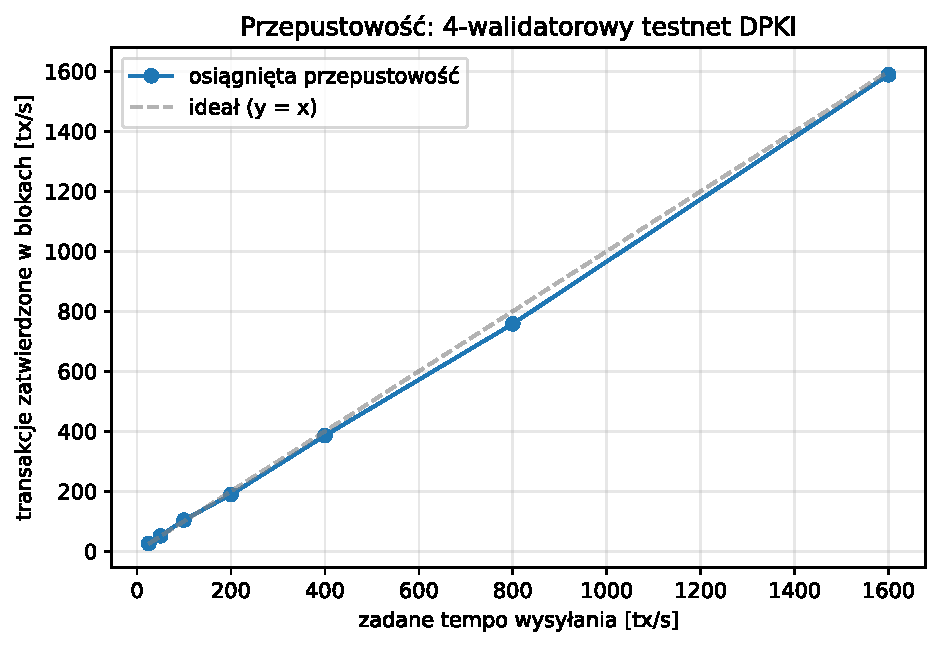
\includegraphics[width=0.85\textwidth]{chart-throughput}
    \caption{Przepustowość osiągnięta w funkcji zadanego tempa obciążenia; linia przerywana oznacza idealną zależność liniową.}
    \label{fig:throughput}
\end{figure}

Najważniejszą obserwacją jest liniowe skalowanie przepustowości w całym zbadanym zakresie - aż do 1588~tx/s przy zadanym tempie 1600~tx/s nie zaobserwowano nasycenia, a wszystkie wysłane transakcje zostały zatwierdzone bez ani jednego odrzucenia. System absorbuje wzrost obciążenia, proporcjonalnie zwiększając liczbę transakcji w bloku (od 31 przy 25~tx/s do niemal dwóch tysięcy przy 1600~tx/s), zamiast wydłużać kolejkę oczekujących. Pierwszego ograniczenia należałoby się spodziewać dopiero powyżej zbadanego zakresu, przy dłuższych falach obciążenia przekraczających domyślną pojemność mempoola. Dla osadzenia tej liczby w kontekście zastosowania: 1588~tx/s odpowiada około 137~milionom operacji na dobę, a więc wartości o rzędy wielkości przewyższającej globalne tempo wystawiania certyfikatów TLS (rzędu kilku milionów dziennie dla największego urzędu). Przepustowość prototypu nie jest zatem czynnikiem ograniczającym dla rozważanego zastosowania.

\subsection{Opóźnienie zatwierdzenia}
\label{subsec:opoznienie}

Opóźnienie zatwierdzenia - czas od wysłania transakcji do jej włączenia w sfinalizowany blok - zmierzono, wysyłając sto transakcji pojedynczo, z przerwą wystarczającą, by każda trafiała w nieskorelowaną fazę interwału bloku. Rozkład wyników podsumowuje tabela~\ref{tab:latencja}, a jego histogram - rysunek~\ref{fig:latency}.

\begin{table}[htbp]
    \centering
    \caption{Statystyki opóźnienia zatwierdzenia transakcji ($n = 100$)}
    \label{tab:latencja}
    \begin{tabular}{l r}
        \hline
        \textbf{Metryka} & \textbf{Wartość [ms]} \\
        \hline
        średnia        & 825 \\
        mediana (p50)  & 813 \\
        percentyl 95 (p95) & 920 \\
        percentyl 99 (p99) & 950 \\
        minimum / maksimum & 784 / 1024 \\
        \hline
    \end{tabular}
\end{table}

\begin{figure}[htbp]
    \centering
    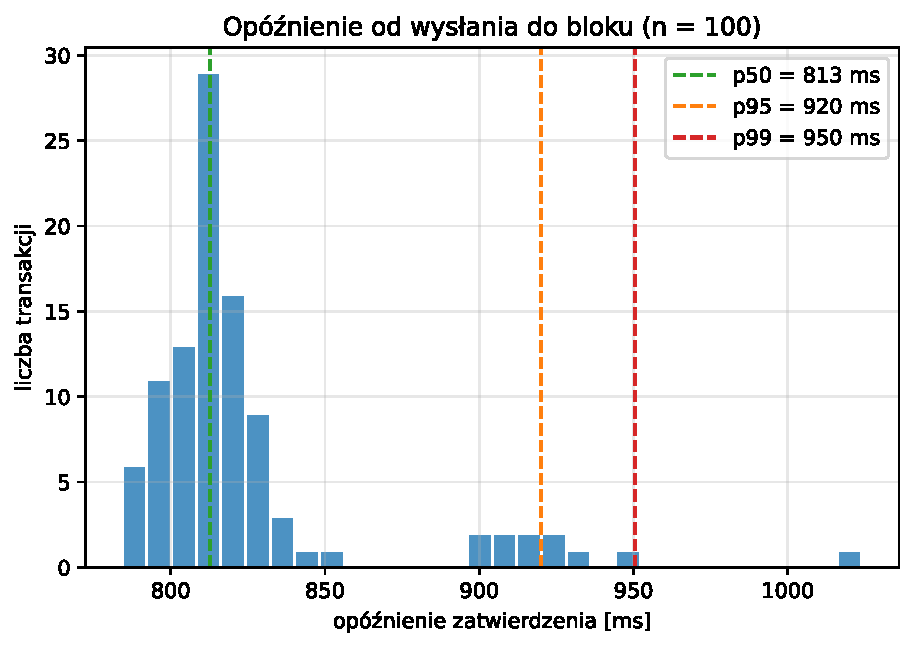
\includegraphics[width=0.85\textwidth]{chart-latency}
    \caption{Histogram opóźnienia zatwierdzenia transakcji wraz z zaznaczonymi percentylami.}
    \label{fig:latency}
\end{figure}

Opóźnienie jest zdominowane przez interwał bloku: transakcja oczekuje średnio około połowy interwału na umieszczenie w propozycji, po czym dochodzi czas rund konsensusu. Mediana 813~ms i niewielki rozrzut między percentylami (różnica p99 i p50 wynosi około 140~ms) świadczą o przewidywalności systemu - opóźnienie jest stabilne, bez długiego ogona. Z punktu widzenia zastosowania kluczowy jest wniosek, że zarówno wystawienie wiązania, jak i jego unieważnienie finalizują się deterministycznie w czasie rzędu jednej sekundy. Stanowi to fundamentalną różnicę względem propagacji unieważnień w klasycznej PKI, liczonej w godzinach lub dniach (sekcja~\ref{sec:crl-ocsp}).

\section{Koszty operacyjne (rozmiar stanu, czas finalizacji)}
\label{sec:koszty}

\subsection{Wzrost stanu}
\label{subsec:wzrost-stanu}

Tempo wzrostu stanu zbadano, wstawiając do drzewa Merkle domeny partiami po dziesięć tysięcy i mierząc po każdej partii rozmiar magazynu oraz średni czas wstawienia. Wyniki przedstawia tabela~\ref{tab:stan}, a zależność rozmiaru stanu od liczby domen - rysunek~\ref{fig:state}.

\begin{table}[htbp]
    \centering
    \caption{Wzrost rozmiaru stanu i czas wstawienia w funkcji liczby domen}
    \label{tab:stan}
    \begin{tabular}{r r r r}
        \hline
        \textbf{Domeny} & \textbf{Magazyn [MB]} & \textbf{Bajtów/domenę} & \textbf{Czas wstawienia [µs]} \\
        \hline
        10\,000  & 156    & $\approx$16\,300 & $\approx$190 \\
        50\,000  & 776    & $\approx$16\,300 & $\approx$180 \\
        100\,000 & 1\,546 & $\approx$16\,200 & $\approx$185 \\
        \hline
    \end{tabular}
\end{table}

\begin{figure}[htbp]
    \centering
    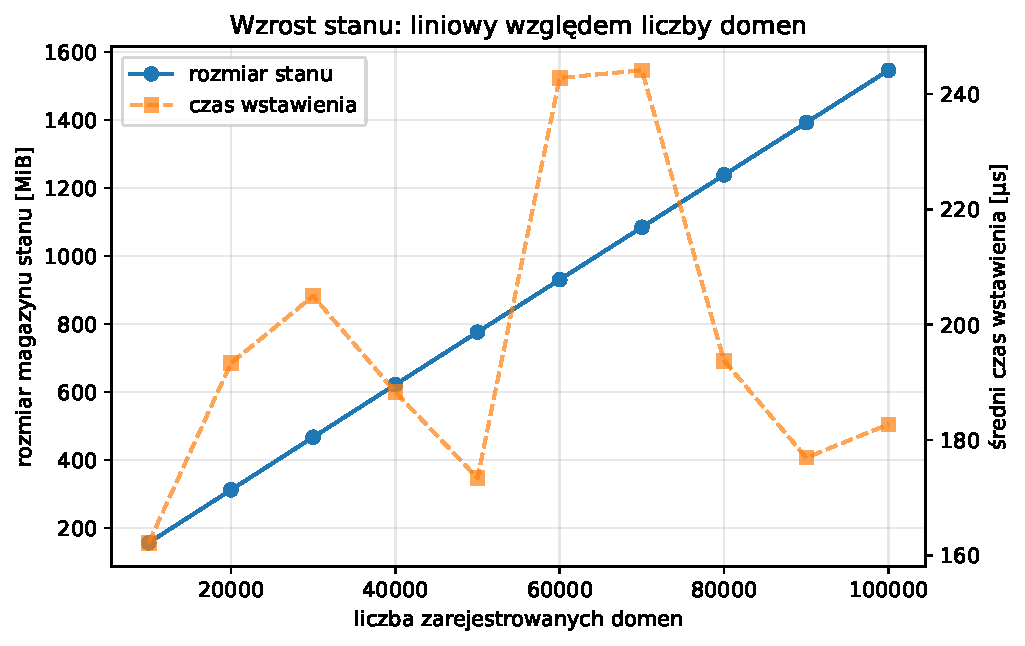
\includegraphics[width=0.85\textwidth]{chart-state-growth}
    \caption{Rozmiar magazynu stanu w funkcji liczby zarejestrowanych domen - zależność liniowa.}
    \label{fig:state}
\end{figure}

Rozmiar stanu rośnie liniowo z liczbą domen, a czas wstawienia pozostaje stały (rzędu 185~µs), niezależny od liczby już zapisanych domen - odzwierciedla to koszt aktualizacji jednej ścieżki w drzewie o stałej głębokości 256. Stały narzut na domenę wymaga jednak uczciwego komentarza, gdyż wartość około 16~kilobajtów znacznie przewyższa rozmiar samego certyfikatu (rzędu 150~bajtów). Różnica nie wynika z rozmiaru danych użytkowych, lecz ze sposobu przechowywania drzewa: w przyjętej, prostej reprezentacji magazyn utrzymuje każdy z węzłów wewnętrznych ścieżki od liścia do korzenia jako osobny wpis. Jest to świadomie zaakceptowany koszt prototypu - produkcyjne implementacje rzadkiego drzewa Merkle stosują kompresję ścieżek (węzły rozszerzające, jak w drzewach Jellyfish Merkle Tree czy Ethereum Merkle Patricia Trie), co redukuje stałą o jeden do dwóch rzędów wielkości, nie zmieniając asymptotycznej złożoności liniowej. Optymalizację tę wskazano jako kierunek dalszych prac (rozdział~\ref{ch:podsumowanie}).

\subsection{Rozmiar i weryfikacja dowodów}
\label{subsec:dowody}

Koszt po stronie strony ufającej wyznacza rozmiar dowodu Merkle oraz czas jego weryfikacji. Zbadano je, próbkując po dwieście losowych dowodów dla trzech rozmiarów drzewa; wyniki zestawia tabela~\ref{tab:dowody}, a zależność rozmiaru dowodu od liczby domen - rysunek~\ref{fig:proof}.

\begin{table}[htbp]
    \centering
    \caption{Rozmiar dowodu i czas weryfikacji w funkcji liczby domen}
    \label{tab:dowody}
    \begin{tabular}{r r r r}
        \hline
        \textbf{Domeny} & \textbf{Dowód włączenia [B]} & \textbf{Dowód nieobecności [B]} & \textbf{Weryfikacja [µs]} \\
        \hline
        1\,000   & 466 & 392 & 27,5 \\
        10\,000  & 572 & 492 & 27,8 \\
        100\,000 & 677 & 605 & 28,0 \\
        \hline
    \end{tabular}
\end{table}

\begin{figure}[htbp]
    \centering
    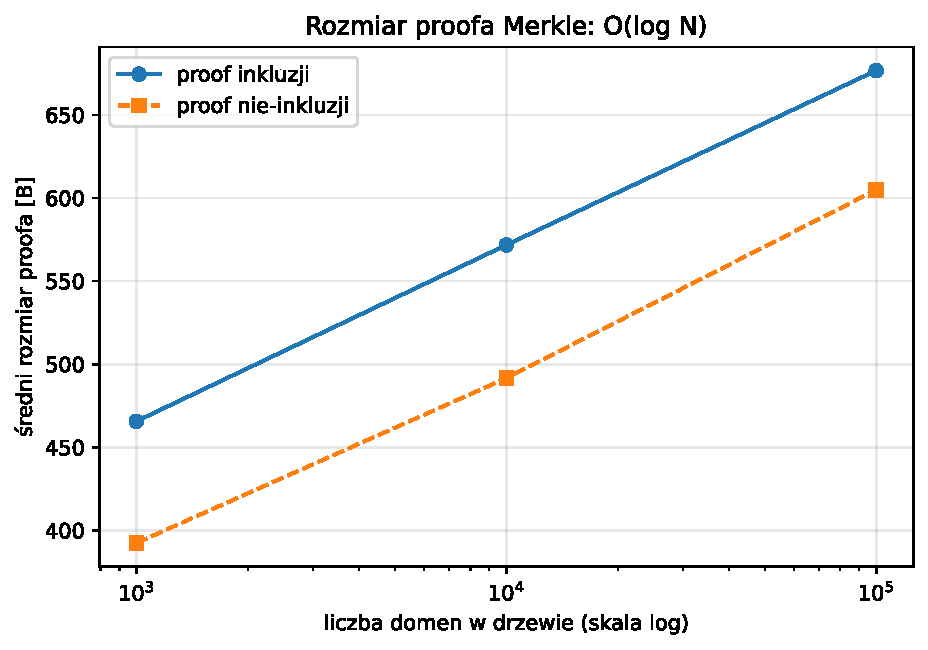
\includegraphics[width=0.85\textwidth]{chart-proof-size}
    \caption{Średni rozmiar dowodu włączenia i nieobecności w funkcji liczby domen (oś pozioma w skali logarytmicznej).}
    \label{fig:proof}
\end{figure}

Rozmiar dowodu rośnie logarytmicznie z liczbą domen - co potwierdza skuteczność kompresji mapą bitową opisanej w sekcji~\ref{subsec:implementacja-merkle} - pozostając w całym zbadanym zakresie poniżej 700~bajtów, podczas gdy czas weryfikacji utrzymuje się na stałym poziomie około 28~mikrosekund. Ekstrapolacja zależności logarytmicznej wskazuje, że nawet dla miliarda domen dowód liczyłby około trzydziestu skrótów rodzeństwa, czyli niewiele ponad kilobajt - wciąż mniej niż typowy łańcuch certyfikatów X.509 (rzędu od dwóch do sześciu kilobajtów). Co istotne, dowód nieobecności ma rozmiar i koszt weryfikacji porównywalny z dowodem włączenia, dzięki czemu weryfikowalna odpowiedź ,,domena nie jest zarejestrowana'' - niedostępna w klasycznej PKI - nie wiąże się z dodatkowym narzutem.

\section{Dyskusja wyników}
\label{sec:dyskusja}

\subsection{Porównanie z klasyczną PKI}
\label{subsec:porownanie-wydajnosc}

Zmierzone charakterystyki pozwalają uzupełnić jakościowe porównanie z rozdziału~\ref{ch:analiza-bezpieczenstwa} o wymiar ilościowy. Zestawienie przedstawia tabela~\ref{tab:porownanie-wyd}.

\begin{table}[htbp]
    \centering
    \caption{Ilościowe porównanie kosztów operacji klasycznej PKI i zaproponowanego systemu}
    \label{tab:porownanie-wyd}
    \begin{tabular}{p{0.28\textwidth} p{0.32\textwidth} p{0.32\textwidth}}
        \hline
        \textbf{Kryterium} & \textbf{Klasyczna PKI (X.509 + CA)} & \textbf{DPKI (zmierzono)} \\
        \hline
        Czas wystawienia & minuty--dni (proces CA) & p50 = 0,81~s (następny blok) \\
        Propagacja unieważnienia & godziny--dni (CRL/OCSP, \emph{soft-fail}) & p50 = 0,81~s, trwała \\
        Rozmiar dowodu ważności & łańcuch certyfikatów 2--6~kB oraz odpowiedź OCSP & dowód 0,5--0,7~kB, weryfikowalny offline \\
        Czas weryfikacji & rząd milisekund (łańcuch podpisów) & 28~µs (dowód) plus weryfikacja podpisu \\
        Dowód nieistnienia & niedostępny & dowód nieobecności rzędu 0,5~kB \\
        Infrastruktura weryfikatora & dostęp do OCSP/CRL w trybie online & zaufany skrót stanu i obliczenie lokalne \\
        \hline
    \end{tabular}
\end{table}

Najwyraźniejsza przewaga ilościowa dotyczy unieważnień: mechanizm propagujący się w czasie jednej sekundy i dający trwały, dowodliwy skutek zastępuje infrastrukturę CRL/OCSP o propagacji liczonej w godzinach i obarczonej praktyką \emph{soft-fail}, która w klasycznym modelu osłabia samą skuteczność unieważnienia (sekcja~\ref{sec:crl-ocsp}). Drugą zauważalną różnicą jest charakter dowodu ważności - zwięzły, weryfikowalny w trybie offline dowód Merkle nie wymaga od weryfikującego łączności z infrastrukturą statusu w momencie weryfikacji, w odróżnieniu od odpytywania respondera OCSP.

\subsection{Skalowalność i jej ograniczenia}
\label{subsec:skalowalnosc}

Zmierzone zależności pozwalają wskazać granice skalowalności systemu. Po stronie konsensusu zasadniczym ograniczeniem jest komunikacja o złożoności kwadratowej względem liczby walidatorów, właściwa protokołom BFT (sekcja~\ref{subsec:bft-tendermint}); wyznacza ona praktyczny pułap rzędu setek walidatorów i sprawia, że dodawanie walidatorów zwiększa odporność, lecz nie przepustowość. Po stronie stanu wzrost jest liniowy i nieograniczony z góry, a istotnym czynnikiem jest tu trwałość unieważnień (sekcja~\ref{subsec:uniewaznienie}): unieważnione wpisy muszą pozostać w stanie, co wyklucza ich usuwanie. Po stronie klienta koszt weryfikacji pozostaje praktycznie stały - logarytmiczny rozmiar dowodu czyni klienta lekkim niezależnie od rozmiaru rejestru. Wreszcie, koszt odzyskiwania stanu przez ponowne odtworzenie historii (sekcja~\ref{subsec:zarzadzanie-stanem}) rośnie liniowo z długością łańcucha - akceptowalny dla prototypu, lecz we wdrożeniu produkcyjnym wymagałby trwałego magazynu stanu. Kierunki łagodzenia tych ograniczeń - kompresja ścieżek drzewa, podział rejestru oraz pełny lekki klient - omówiono w rozdziale~\ref{ch:podsumowanie}.

\subsection{Wnioski}
\label{subsec:wnioski-eksperymenty}

Przeprowadzone pomiary prowadzą do spójnego wniosku: zaproponowany system osiąga przepustowość i opóźnienie o rzędy wielkości lepsze niż procesy klasycznej PKI tam, gdzie ma to największe znaczenie dla bezpieczeństwa - w propagacji unieważnień - przy koszcie w postaci stałego narzutu pamięciowego na domenę oraz ograniczenia skali zbioru walidatorów. Koszt ten jest bezpośrednią konsekwencją zamiany zaufanej trzeciej strony na replikowaną maszynę stanów: bezpieczeństwo i transparentność uzyskuje się tu przez redundancję i jawność, nie zaś przez zaufanie do pojedynczego podmiotu. Wartości bezwzględne, uzyskane w środowisku jednomaszynowym, należy traktować jako orientacyjne, jednak zaobserwowane relacje - liniowy wzrost stanu, logarytmiczny rozmiar dowodu, stały koszt weryfikacji - są niezależne od środowiska i potwierdzają praktyczną wykonalność oraz skalowalność przyjętego podejścia w zakresie istotnym dla zastosowania.
